\documentclass[11pt]{article}

\usepackage[T1]{fontenc}
\usepackage{lmodern}
\usepackage[spanish,mexico,es-noshorthands,es-nosectiondot]{babel}
\spanishplainpercent
\usepackage[margin=2.5cm]{geometry}
\usepackage{amsmath}
\usepackage{amssymb}
\usepackage{booktabs}
\usepackage{array}
\usepackage{tabularx}
\usepackage{longtable}
\usepackage{graphicx}
\usepackage{float}
\usepackage[section]{placeins}
\usepackage[hidelinks]{hyperref}

% Flotantes: más espacio para tablas en páginas con texto y páginas de flotantes alineadas arriba.
\renewcommand{\topfraction}{0.85}
\renewcommand{\bottomfraction}{0.7}
\renewcommand{\textfraction}{0.1}
\renewcommand{\floatpagefraction}{0.7}
\makeatletter
\setlength{\@fptop}{0pt}
\makeatother

\hypersetup{pdftitle={Lluvia y emergencias urbanas en Hermosillo: reporte técnico}}

% Rutas e identificadores en monoespaciado, con cortes de línea en / . _ y -.
\newcommand{\cod}[1]{\nolinkurl{#1}}
\expandafter\def\expandafter\UrlBreaks\expandafter{\UrlBreaks\do\_\do\-}

\renewcommand*{\descriptionlabel}[1]{\hspace\labelsep\normalfont #1}
\newcolumntype{L}[1]{>{\raggedright\arraybackslash}p{#1}}
\newcolumntype{Y}{>{\raggedright\arraybackslash}X}
\renewcommand{\arraystretch}{1.15}

% Las cifras de resultados salen de las salidas guardadas de
% notebooks/08-exploracion-redefinicion.ipynb y notebooks/09-historia-lluvia-911.ipynb.
% Las dimensiones de los datos salen de una inspección de solo lectura de data/raw y
% data/processed (corte del 15 de noviembre de 2026).

\begin{document}

\begin{center}
  {\LARGE Lluvia y emergencias urbanas en Hermosillo\par}
  \vspace{0.3em}
  {\large Reporte técnico: datos, definiciones y decisiones\par}
  \vspace{0.8em}
  Nombre del integrante 1 · correo@pendiente · LinkedIn o GitHub pendiente\\
  Nombre del integrante 2 · correo@pendiente · LinkedIn o GitHub pendiente\\
  Nombre del integrante 3 · correo@pendiente · LinkedIn o GitHub pendiente\\
  Nombre del integrante 4 · correo@pendiente · LinkedIn o GitHub pendiente\\[0.5em]
  Ingeniería de características, maestría en ciencia de datos. Corte: 15 de noviembre de 2026.
\end{center}

\section*{Resumen técnico}

Se cruzó la precipitación diaria de Open-Meteo \cite{zippenfenig2023} en un punto de Hermosillo (3,195 días, enero de 2018 a septiembre de 2026) con 4,176 llamadas al 911 \cite{marcelinux2025} de 28 tipos de incidente ligados al agua y al terreno, seleccionadas de 2,297,081 llamadas crudas, y con dos fuentes de contraste: 39,018 reportes del Bachómetro \cite{bachometro} y 5,200 publicaciones de Agua de Hermosillo \cite{aguah}. Las llamadas se ubicaron en las 762 colonias de la ciudad del DCAH 2025 \cite{inegidcah} por nombre normalizado (67.0\% de las llamadas) y se midió la distancia de cada colonia al cauce más cercano de la Red Hidrográfica 1:50\,000 \cite{inegired}. Con un estudio de evento dentro de junio a octubre (ventana de 8 días, umbral de 10~mm), el conteo diario de llamadas por inundación tras lluvia es 21.70 veces el de días secos; terreno 3.66 y drenaje 2.47. Baches (0.97 dentro del mismo mes) y emergencias de Agua de Hermosillo (0.99) no responden. Este documento dimensiona las fuentes, fija las definiciones operativas con su notación, resume la exploración E1 a E8 y los resultados operativos, y rastrea cada cifra del reporte ejecutivo hasta la salida que la produce.

\subsection*{Relación con el reporte ejecutivo}

El reporte ejecutivo (\cod{docs/reporte/reporte.tex}) responde, en lenguaje no técnico y para Protección Civil municipal y el C5, cuatro preguntas: cuándo llama la ciudad al 911 por la lluvia, qué piden y a qué hora, dónde, y si pasa lo mismo con baches y agua potable. Este reporte técnico responde de dónde sale cada cifra de ese documento, con qué definición se calculó, qué decisiones de limpieza y de alcance la sostienen y qué tan firme es. La sección~\ref{sec:traza} contiene la tabla de trazabilidad.

\section{Fuentes y datasets}
\label{sec:fuentes}

Las tablas~\ref{tab:crudas-origen} y \ref{tab:crudas-forma} describen las fuentes crudas y la tabla~\ref{tab:procesados} los datasets procesados. Los tamaños son bytes en disco divididos entre $10^6$; filas y columnas se contaron sobre los archivos del corte. Las dimensiones del DCAH, el Marco Geoestadístico, la Red Hidrográfica y Facebook vienen de \cod{docs/cinco_v_datos.md} y sus tamaños coinciden con los actuales en disco; las demás se contaron directamente.

\begin{table}[!htbp]
  \centering
  \footnotesize
  \caption{Fuentes crudas: origen, licencia, formato y tamaño. MB: tamaño en disco de los archivos descargados, sin \cod{FUENTE.txt}.}
  \label{tab:crudas-origen}
  \begin{tabularx}{\textwidth}{L{2.6cm} Y L{2.3cm} L{2.1cm} r}
    \toprule
    Fuente & Origen & Licencia & Formato & MB \\
    \midrule
    Llamadas al 911 & Hugging Face, Marcelinux: \cod{huggingface.co/datasets/Marcelinux/llamadas911_colonias_hermosillo_2018_2025} (archivo \cod{213.xlsx}) & CC-BY-4.0 & Excel, una hoja por año & 52.8 \\
    Precipitación & Open-Meteo, API de archivo histórico: \cod{archive-api.open-meteo.com/v1/archive} & CC-BY-4.0 & JSON & 0.1 \\
    Bachómetro & H. Ayuntamiento de Hermosillo: \cod{bachometro.hermosillo.gob.mx/mapa/ajax} & no declarada & JSON, uno por año & 8.2 \\
    DCAH 2025 & INEGI, paquete nacional, miembro \cod{26_sonora.zip} bajado por rango & Términos de Libre Uso del INEGI & Shapefile, CSV, TXT & 15.5 \\
    Marco Geoestadístico 2025, capa \cod{26e} & INEGI, paquete de Sonora, solo la capa de ejes de vialidad & Términos de Libre Uso del INEGI & Shapefile & 66.3 \\
    Red Hidrográfica 1:50\,000, ed. 2.0 & INEGI, cuatro subcuencas: La Poza, R. Sonora-Hermosillo, La Manga, R. San Miguel & Términos de Libre Uso del INEGI & Shapefile, 5 capas por subcuenca & 50.8 \\
    Agua de Hermosillo & Página oficial de Facebook, extraída con un scraper de Apify; imágenes y OCR con PaddleOCR-VL 1.6 (snapshot v1, \cod{data/SNAPSHOT.md}) & no declarada; snapshot privado & CSV, imágenes, CSV de OCR & 210.0 \\
    \bottomrule
  \end{tabularx}
\end{table}

\begin{table}[!htbp]
  \centering
  \footnotesize
  \caption{Fuentes crudas: periodo, granularidad, dimensiones, job de ingesta y ruta. Los jobs están en \cod{project_name/jobs/} y los corre \texttt{make download}, salvo Facebook, que es un insumo congelado.}
  \label{tab:crudas-forma}
  \begin{tabularx}{\textwidth}{L{2.2cm} L{2.3cm} Y L{2.4cm} L{3.9cm}}
    \toprule
    Fuente & Periodo & Granularidad temporal y espacial & Registros $\times$ columnas & Job y ruta \\
    \midrule
    Llamadas al 911 & 2018-01-01 a 2025-09-30 & Una llamada con fecha y hora entera; ubicación solo como nombre de colonia en texto libre, sin coordenadas & 2,297,081 $\times$ 4 (8 hojas; 475 tipos de incidente) & \cod{ingest_llamadas_911_job}; \cod{data/raw/llamadas911/llamadas_911_hermosillo.xlsx} \\
    Precipitación & 2018-01-01 a 2026-09-30 & Diaria en hora local (\cod{America/Hermosillo}); un punto solicitado (29.0892, $-110.9613$); la API devolvió las coordenadas 29.06854, $-110.975876$ y elevación de 210~m & 3,195 días $\times$ 2 variables (\cod{precipitation_sum}, \cod{precipitation_hours}) & \cod{ingest_precipitacion_job}; \cod{data/raw/precipitacion/precipitacion_hermosillo.json} \\
    Bachómetro & 2021-09-17 a 2026-10-03 & Un reporte con fecha y punto (latitud, longitud) & 39,106 $\times$ 7 (el procesado del 28 de septiembre de 2026 tiene 39,018) & \cod{ingest_baches_job}; \cod{data/raw/bachometro/baches_2021.json} a \cod{baches_2026.json} \\
    DCAH 2025 & Edición 2025, actualización 11/2025 & Estática; polígono por asentamiento, EPSG:6372 & 2,699 asentamientos de Sonora $\times$ 10 & \cod{ingest_dcah_job}; \cod{data/raw/inegi/dcah/dcah_2025_26_sonora.zip} \\
    Marco Geoestadístico & Edición 2025 & Estática; línea por tramo de calle, EPSG:6372 & 229,303 tramos $\times$ 11 & \cod{ingest_mg_streets_job}; \cod{data/raw/inegi/mg/} \\
    Red Hidrográfica & Segmentos fechados de 1998 a 2010 & Estática; líneas, puntos y polígonos, EPSG:4019 & 48,023 geometrías; 3 a 22 atributos por capa & \cod{ingest_subcuencas}; \cod{data/raw/inegi/subc_*/} \\
    Agua de Hermosillo & 2020-12-07 a 2026-09-14 & Una publicación con fecha y hora; lugares solo en texto & 5,200 publicaciones en 7 CSV; 3,203 imágenes & sin job de descarga; \cod{data/external/} \\
    \bottomrule
  \end{tabularx}
\end{table}

\begin{table}[!htbp]
  \centering
  \footnotesize
  \caption{Datasets procesados. Todos los produce \texttt{make data}. Uso: papel en la pregunta final. Las rutas son relativas a \cod{data/processed/}.}
  \label{tab:procesados}
  \begin{tabularx}{\textwidth}{L{3.6cm} L{2.0cm} r L{2.0cm} L{3.0cm} Y}
    \toprule
    Dataset y ruta & Filas $\times$ columnas & MB & Periodo & Job & Uso \\
    \midrule
    \cod{llamadas_911/llamadas_911_hermosillo.csv} & 4,176 $\times$ 5 & 0.27 & 2018-01-05 a 2025-09-30 & \cod{process_llamadas_911_job} & Serie principal: 28 tipos, 5 grupos \\
    \cod{precipitacion/precipitacion_hermosillo.csv} & 3,195 $\times$ 6 & 0.10 & 2018-01-01 a 2026-09-30 & \cod{process_precipitacion_job} & Variable explicativa \\
    \cod{aguah/colonias_hermosillo.csv} y \cod{.gpkg} & 783 $\times$ 10, más polígono & 0.09 y 0.75 & DCAH 2025 & \cod{process_colonias_hermosillo_job} & Ubicación; 762 asentamientos con \cod{locality_code} 0001 \\
    \cod{inegi/hidrografia_hermosillo/subc_hermosillo.gpkg} & capas \cod{hl} 46,518; \cod{dr} 36; \cod{subc} 4; \cod{ha} 744; \cod{to} 124 & 35.89 & 1998 a 2010 & \cod{process_subcuencas_job} & Distancia al cauce (capa \cod{hl}) y cauces del mapa \\
    \cod{inegi/hidrografia_hermosillo/hidrografia_cd_hermosillo.gpkg} & capas \cod{hl} 437; \cod{dr} 1; \cod{subc} 4; \cod{ha} 16; \cod{to} 5 & 0.47 & 1998 a 2010 & \cod{process_hidrografia_cd_hermosillo_job} & No lo leen los notebooks 08 y 09 \\
    \cod{bachometro/baches_hermosillo.csv} & 39,018 $\times$ 10 & 5.53 & 2021-09-17 a 2026-09-28 & \cod{process_baches_job} & Contraste \\
    \cod{aguah/publicaciones_aguah.csv} & 5,200 $\times$ 32 & 4.22 & 2020-12-07 a 2026-09-14 & \cod{process_publicaciones_aguah_job} & Contraste y texto \\
    \cod{aguah/ubicaciones_aviso.csv} & 16,261 $\times$ 8 & 1.34 & igual que las publicaciones & \cod{process_ubicaciones_aviso_job} & No entra; contexto del tablero de agua potable \\
    \bottomrule
  \end{tabularx}
\end{table}

Las dos fuentes de contraste no entran a la pregunta final, pero cumplen un papel de prueba: si la lluvia moviera también los reportes de baches o las emergencias de agua potable, el pronóstico serviría para esos servicios. La exploración E1 a E3 (sección~\ref{sec:eda}) muestra que no es así, y por eso quedan como contraste y, en el caso de Agua de Hermosillo, como evidencia de texto.

Sobre la precipitación: no se confirmó qué modelo usa la API de archivo de Open-Meteo para este punto. Se describe como la combinación por defecto de reanálisis de Open-Meteo; es una malla, no una estación, y no se afirma un tamaño de celda. ERA5-Land \cite{munozsabater2021} es uno de los reanálisis que combina Open-Meteo, pero no se confirmó que sea el de este punto; por eso \cod{params.yml}, \cod{FUENTE.txt}, \cod{docs/redefinicion.md}, el notebook 08 y la figura~\ref{fig:hallazgo} ya no la rotulan como ERA5.

\section{Preprocesamiento por fuente}
\label{sec:prep}

\subsection{Llamadas al 911}

\begin{enumerate}
  \item Carga: \cod{load_llamadas_911} (\cod{project_name/features.py}) concatena las 8 hojas del Excel con el lector \cod{calamine}: 2,297,081 filas $\times$ 4 columnas (\cod{COLONIA}, \texttt{TIPO DE INCIDENTE}, \cod{FECHA}, \cod{HORA}).
  \item Nulos: \cod{clean_llamadas_911} quita las filas con algún nulo; hay 7 nulos por columna y quedan 2,297,074 filas.
  \item Selección de tipos: se conservan los tipos de \cod{GRUPOS_INCIDENTE_911}, 34 cadenas del catálogo de 475, elegidas a mano en \cod{notebooks/AAMM/00} y agrupadas en 5 grupos: \cod{inundacion_directa} (4 cadenas), \cod{fenomeno_hidrometeorologico} (10), \cod{drenaje_y_red_de_agua} (7), \cod{ahogamiento_acuaticos} (5) y \cod{terreno} (8). Quedan 4,176 llamadas, el 0.2\% de las crudas. Motivo: la pregunta trata de emergencias urbanas ligadas al agua y al terreno, no del total de la demanda del 911.
  \item Unificación por ortografía: \cod{process_llamadas_911_job} reemplaza ``ÁRBOL CAÍDO O POR CAER'' (45 llamadas) por ``ARBOL CAÍDO O POR CAER'' y ``VIALIDAD EN MAL ESTADO-BACHES'' (28) por ``VIALIDAD EN MAL ESTADO'', ``INUNDACIÓN'' (24) por ``INUNDACIONES'' (399), ``ALCANTARILLA-REGISTRO SIN TAPA'' (16) por ``ALCANTARILLA SIN TAPA'' (990), ``AHOGAMIENTO-SUMERSIÓN'' (4) por ``AHOGAMIENTO'' (74) y la variante de hundimientos ``EN SUELO'' (2) por la mayoritaria (365). Cada par pertenece al mismo grupo, así que los totales por grupo no cambian. Las 34 cadenas quedan en 28 tipos. ``HURACANES-CAÍDA DE ÁRBOL'' no se unifica con árbol caído: es una categoría del protocolo de huracanes. La función es \cod{unify_tipos_incidente}, con pruebas en \cod{tests/test_process_llamadas_911_job.py}.
  \item Columnas: se renombran a \cod{colonia}, \cod{tipo_incidente}, \cod{fecha}, \cod{hora} (entero de 0 a 23) y se agrega \cod{grupo_incidente}. Resultado por grupo: terreno 2,545; drenaje 1,066; inundación 454; ahogamiento 84; fenómeno hidrometeorológico 27.
  \item Exclusión de ahogamientos en la historia: \cod{rain_related_calls} (\cod{project_name/water_events.py}) quita el grupo \cod{ahogamiento_acuaticos} en el notebook 09, porque esos incidentes no dependen de la lluvia en la ciudad. Quedan 4,092 llamadas de 27 tipos. El notebook 08 trabaja por grupo y no necesita esa exclusión.
\end{enumerate}

\subsection{Emparejamiento de colonias del 911}

El 911 no trae coordenadas. \cod{match_colonia} asigna \cod{colonia_id} así:

\begin{enumerate}
  \item Catálogo: asentamientos del DCAH con \cod{locality_code} igual a \cod{0001}, la ciudad de Hermosillo (762 de 783 del municipio; \cod{load_colonias}).
  \item Normalización: \cod{normalize_name} (\cod{project_name/text.py}) quita acentos con NFKD, pasa a mayúsculas, sustituye por espacio todo lo que no sea letra A a Z, dígito o espacio, y colapsa espacios. Se aplica igual al nombre del 911 y al nombre del INEGI.
  \item Unicidad: solo se aceptan nombres normalizados que corresponden a un único asentamiento en la ciudad. Los 762 asentamientos tienen 742 nombres normalizados; 724 son únicos y 18 se repiten en 38 asentamientos. Un nombre repetido no se asigna, para no repartir una llamada entre colonias homónimas.
\end{enumerate}

Cobertura: 67.0\% de las 4,176 llamadas recibe colonia única (salida \cod{quality_table} del notebook 08); quedan sin colonia 1,380 (33.0\%, \cod{docs/eda.md}), de ellas 57 con el texto ``SIN COLONIA''. Las llamadas ubicadas caen en 314 colonias. Los análisis temporales usan todas las llamadas; los análisis por colonia, solo las ubicadas.

\subsection{Bachómetro}

\cod{process_baches_job} concatena los seis JSON anuales, convierte latitud, longitud y fecha, agrega \cod{year} (el archivo de origen), \cod{date_mx} e \cod{id_row}. No depura filas. La exploración midió tres anomalías (salida \cod{quality_table}, notebook 08):

\begin{itemize}
  \item \cod{year} distinto del año de \cod{date} en 1,584 filas: \cod{year} es el archivo de descarga, no la fecha del reporte. Decisión: usar \cod{date}.
  \item 511 reportes fuera del recuadro de la ciudad (latitud 28.8 a 29.3, longitud $-111.2$ a $-110.8$). Decisión: excluir de mapas. \cod{docs/cinco_v_datos.md} cuenta 266 con otro recuadro (\cod{HERMOSILLO_BOUNDS}: latitud 27.5 a 30.5, longitud $-113.0$ a $-110.0$).
  \item 152 reportes repetidos en coordenada, fecha y texto (doble envío). Decisión: no depurar.
\end{itemize}

En los conteos diarios de E2 entran las 39,018 filas dentro de la ventana de cobertura, incluidos los puntos fuera del recuadro y los repetidos. El cruce espacial de baches a colonia (\cod{add_colonia_bache_with_gpkg}) se conserva para el tablero; el cruce por nombre (\cod{add_colonia_name_to_bache_job}) se desechó porque su salida es nula en todas las filas (\cod{docs/redefinicion.md}).

\subsection{Agua de Hermosillo}

\cod{process_publicaciones_aguah_job} une cada publicación con su OCR (1:1 por \cod{postId}), convierte la hora a \cod{America/Hermosillo} y clasifica el tipo de evento con \cod{classify_events} (\cod{project_name/text.py}) sobre el texto y el OCR en minúsculas. Reglas, en orden de prioridad creciente (gana la última que coincide): \cod{pipas} (``pipa''), \cod{emergencia} (fuga, ruptura, emergencia, falla eléctrica, desabasto), \cod{corte_programado} (programad, suspensión o corte del servicio) y \cod{restablecimiento} (restablecido, se normalizó, reanudó, concluyó la reparación, entre otras). Antes de clasificar se borran las promesas de restablecimiento futuro (``será restablecido''). Lo que no coincide queda como \cod{otro}. Resultado: 3,919 \cod{otro}, 811 \cod{emergencia}, 295 \cod{corte_programado}, 134 \cod{restablecimiento} y 41 \cod{pipas}.

Ventana útil: \cod{COVERAGE} fija enero de 2021 a julio de 2026. Diciembre de 2020 está incompleto, y agosto y septiembre de 2026 tienen 36 y 16 publicaciones contra 120 a 132 en los meses previos (\cod{docs/eda.md}), probable corte de la última exportación del scraper.

\subsection{Red hidrográfica}

\cod{process_subcuencas_job} consolida las cinco capas de las cuatro subcuencas en \cod{subc_hermosillo.gpkg} (EPSG:4019). Para la distancia al cauce, \cod{stream_distance} reproyecta la capa \cod{hl} y las colonias a EPSG:6372 (metros), forma la unión de las 762 colonias de la ciudad, la amplía con un buffer de 5~km y conserva los tramos que la intersecan: 1,932 de 46,518. Es el mismo criterio de \cod{notebooks/AAMM/07}. El recorte \cod{hidrografia_cd_hermosillo.gpkg} (437 tramos dentro de la mancha urbana) no se usa para la distancia, porque dejaría fuera los cauces que corren justo afuera del borde.

\subsection{Precipitación}

\cod{ingest_precipitacion_job} arma la URL con los parámetros de \cod{params.yml} (\cod{sources.open_meteo}) y descarga todo el rango en una petición: latitud 29.0892, longitud $-110.9613$, del 2018-01-01 al 2026-09-30, variables diarias \cod{precipitation_sum} y \cod{precipitation_hours}, zona \cod{America/Hermosillo}. \cod{process_precipitacion_job} produce una fila por día con \cod{date}, \cod{precipitation_mm}, \cod{precipitation_hours}, \cod{year}, \cod{month} e \cod{is_rain_day} ($\geq 1$~mm). No hay nulos ni días faltantes: 3,195 días, 309 con 1~mm o más, 63 con 10~mm o más y 30 con 20~mm o más; el máximo es 65.6~mm (2025-09-05). Las pruebas del job están en \cod{tests/test_precipitacion_jobs.py}.

\section{Datos faltantes y cobertura}
\label{sec:cobertura}

\begin{table}[!htbp]
  \centering
  \small
  \caption{Cobertura de cada fuente (salida \cod{coverage_table} del notebook 08) y ventana de meses completos que usa el análisis (\cod{COVERAGE} en \cod{water_events.py}).}
  \label{tab:cobertura}
  \begin{tabular}{lrlll}
    \toprule
    Fuente & Filas & Primer registro & Último registro & Ventana del análisis \\
    \midrule
    Lluvia & 3,195 & 2018-01-01 & 2026-09-30 & 2018-01-01 a 2026-09-30 \\
    911 & 4,176 & 2018-01-05 & 2025-09-30 & 2018-01-01 a 2025-09-30 \\
    Baches & 39,018 & 2021-09-17 & 2026-09-28 & 2022-01-01 a 2026-09-30 \\
    Agua de Hermosillo & 5,200 & 2020-12-07 & 2026-09-14 & 2021-01-01 a 2026-07-31 \\
    \bottomrule
  \end{tabular}
\end{table}

\begin{itemize}
  \item Ventanas comunes: lluvia y 911, enero de 2018 a septiembre de 2025 (la que usan la historia y el estudio de evento del 911); lluvia, 911 y baches, enero de 2022 a septiembre de 2025.
  \item Huecos: ninguna fuente tiene un mes sin registros dentro de su periodo (salida \cod{gaps} del notebook 08, listas vacías). Agua de Hermosillo no tiene publicaciones entre el 5 y el 19 de abril de 2024, en la frontera entre dos exportaciones del scraper (13 días según \cod{docs/eda.md}; 14 según \cod{docs/cinco_v_datos.md}).
  \item 911 sin colonia: 33.0\% de las llamadas (1,380), 57 con ``SIN COLONIA''. Mecanismo: nombre libre del operador y localidades fuera de la ciudad. Tratamiento: fuera de los análisis por colonia.
  \item Cambio de catálogo: \cod{fenomeno_hidrometeorologico} tiene 0 llamadas de 2018 a 2024 y 27 en 2025 (tabla~\ref{tab:anual-grupo}). Es un catálogo nuevo, no un fenómeno nuevo; no se compara entre años.
  \item Lluvia: sin nulos. Baches: sin nulos, con las anomalías de la sección~\ref{sec:prep}.
\end{itemize}

\begin{table}[!htbp]
  \centering
  \small
  \caption{Llamadas al 911 por año y grupo (salida \cod{calls_by_year}, notebook 08). 2025 llega a septiembre.}
  \label{tab:anual-grupo}
  \begin{tabular}{lrrrrr}
    \toprule
    Año & Ahogamiento & Drenaje & Fenómeno hidromet. & Inundación & Terreno \\
    \midrule
    2018 & 11 & 108 & 0 & 153 & 232 \\
    2019 & 10 & 110 & 0 & 63 & 242 \\
    2020 & 7 & 53 & 0 & 3 & 168 \\
    2021 & 19 & 154 & 0 & 71 & 327 \\
    2022 & 15 & 205 & 0 & 90 & 515 \\
    2023 & 10 & 157 & 0 & 7 & 271 \\
    2024 & 5 & 135 & 0 & 17 & 381 \\
    2025 & 7 & 144 & 27 & 50 & 409 \\
    \bottomrule
  \end{tabular}
\end{table}

\section{Definiciones operativas}
\label{sec:defs}

Notación común. Sea $t$ un día y $R_t$ la precipitación de ese día en mm. Sea $Y^{(s)}_t$ el número de registros de la serie $s$ (un grupo o tipo del 911, baches o emergencias de Agua de Hermosillo) con fecha $t$; los días sin registros valen 0 dentro de la ventana de cobertura de la serie (tabla~\ref{tab:cobertura}). $\operatorname{mes}(t)$ y $\text{año}(t)$ son el mes y el año calendario de $t$.

\begin{description}
  \item[Temporada.] $\mathcal{T}=\{t:\operatorname{mes}(t)\in\{6,7,8,9,10\}\}$, junio a octubre (\cod{RAINY_MONTHS}). En la ventana del 911 son 1,193 días.
  \item[Ventana de respuesta.] Con $W=8$ días (\cod{RESPONSE_DAYS}),
  \[ M_t=\max_{0\le j\le W-1} R_{t-j}, \]
  donde $M_t$ es la lluvia máxima del día y los siete anteriores (\cod{response_window}). Un día está en la ventana de respuesta de una lluvia si $M_t\geq\tau$.
  \item[Umbral y día seco.] $\tau=10$~mm (\cod{RAIN_EVENT_MM}) y $\delta=1$~mm (\cod{DRY_MM}). Día húmedo: $M_t\ge\tau$. Día seco: $M_t<\delta$, sin lluvia de 1~mm en los 8 días. En la tabla de intensidad, el día seco es en cambio $R_t<\delta$ el mismo día; la sección~\ref{sec:limites} discute la diferencia.
  \item[Razón de temporada.] Con $H=\{t\in\mathcal{T}:M_t\ge\tau\}$ y $S=\{t\in\mathcal{T}:M_t<\delta\}$,
  \[ Q^{(s)}=\frac{\bar{Y}^{(s)}_H}{\bar{Y}^{(s)}_S},\qquad \bar{Y}^{(s)}_A=\frac{1}{|A|}\sum_{t\in A}Y^{(s)}_t, \]
  donde $Q^{(s)}$ es cuántas veces el conteo medio tras lluvia supera al de días secos de la misma temporada (\cod{event_study}).
  \item[Control dentro del mismo mes.] Para cada mes calendario $m$ de cada año, $H_m=\{t\in m:M_t\ge\tau\}$ y $S_m=\{t\in m:M_t<\delta\}$, sobre todos los meses del año y no solo la temporada. Sea $\mathcal{M}$ el conjunto de meses con $H_m$ y $S_m$ no vacíos (meses comparables). Se reportan $|\mathcal{M}|$, el número de meses con $\bar{Y}_{H_m}>\bar{Y}_{S_m}$ y con $\bar{Y}_{H_m}<\bar{Y}_{S_m}$, y
  \[ Q_{\text{mes}}=\frac{\sum_{m\in\mathcal{M}}\bar{Y}_{H_m}}{\sum_{m\in\mathcal{M}}\bar{Y}_{S_m}}, \]
  el cociente de las medias de los promedios mensuales (\cod{within_month_ratio}). Se cuentan meses en lugar de promediar razones porque muchos meses secos tienen 0 llamadas por inundación.
  \item[Spearman con rezagos.] $r_s(k)$ es la correlación de Spearman, la de Pearson entre los rangos, entre $R_t$ y $Y^{(s)}_{t+k}$, para $k\in\{0,1,2,3,7,14,30\}$, sobre los días con ambas series definidas (\cod{lagged_spearman}).
  \item[Participación de julio a septiembre.] Con $N_{y,m}$ los registros del año $y$ en el mes $m$,
  \[ \pi_y=100\,\frac{\sum_{m=7}^{9}N_{y,m}}{\sum_{m=1}^{12}N_{y,m}}, \]
  solo para años completos (\cod{monthly_share}). Una serie sin estacionalidad da $\pi_y\approx 25.0\%$.
  \item[Categorías de intensidad.] Por la lluvia del mismo día $R_t$: seco ($R_t<1$), 1 a 10~mm, 10 a 20~mm, 20 a 40~mm y 40~mm o más, con cortes en 0.99, 9.99, 19.99 y 39.99 (\cod{INTENSITY_BINS}); la lluvia viene con resolución de 0.1~mm. Solo días de $\mathcal{T}$ en la ventana del 911 (\cod{calls_by_intensity}).
  \item[Día malo.] Para la categoría $c$, el percentil 90 de $Y_t$ entre sus días, $P_{90}(c)$, con interpolación lineal (\cod{quantile(0.9)} de pandas): solo 1 de cada 10 días de la categoría lo supera.
  \item[Evento aislado.] Con $\tau_E=20$~mm (\cod{EVENT_MM}),
  \[ E=\{t:R_t\ge\tau_E,\ \max(R_{t-1},R_{t-2},R_{t-3})<\tau\}, \qquad C(k)=\frac{1}{|E|}\sum_{e\in E}Y_{e+k},\quad k=-3,\dots,7, \]
  donde $C(k)$ es la curva de evento (\cod{event_curve}). $E$ no se restringe a la temporada (7 de los 13 eventos caen fuera de junio a octubre, salida \cod{eventos_en_temporada}), así que la referencia es el día seco de todo el año, $\bar{Y}$ sobre $\{t:R_t<\delta\}$, con valor 1.04.
  \item[Llamadas extra por tipo.] Para el tipo $j$, $x_j=\bar{Y}^{(j)}_H-\bar{Y}^{(j)}_S$, con $H$ y $S$ de la razón de temporada (\cod{extra_calls_by_type}).
  \item[Perfil por hora.] Con $h_i\in\{0,\dots,23\}$ la hora de la llamada $i$ y $t_i$ su día, $p_h=100\,|\{i:h_i=h,\ R_{t_i}\ge\tau\}|\,/\,|\{i:R_{t_i}\ge\tau\}|$ para el día de lluvia, y lo mismo con $M_{t_i}<\delta$ para el día seco; ambos sobre todos los meses (\cod{hour_profile}). Madrugada: $\sum_{h=1}^{5}p_h$, de la 1:00 a las 5:59.
  \item[Distancia al cauce.] Para la colonia $c$ con centroide $g_c$ en EPSG:6372, $d_c=\min_{\ell\in L}\operatorname{dist}(g_c,\ell)$, donde $L$ son los tramos de la capa \cod{hl} que intersecan la unión de las colonias de la ciudad ampliada 5~km (\cod{stream_distance}).
  \item[Persistencia entre años.] Con $n_{c,a}$ las llamadas ubicadas de la colonia $c$ en el año $a$ (tras lluvia, $M_t\ge\tau$, o todas), la persistencia entre los años $a$ y $b$ es $r_s$ entre los vectores $(n_{c,a})_c$ y $(n_{c,b})_c$, sobre las colonias con al menos una llamada en el conjunto, para los pares 2018-2019, 2019-2021, 2021-2022 y 2022-2025.
  \item[Temporadas con llamadas por colonia.] Con $\mathcal{L}_c$ las llamadas ubicadas en la colonia $c$ y $M_{t_i}\ge\tau$,
  \[ T_c=\bigl|\{\text{año}(t_i):i\in\mathcal{L}_c\}\bigr|,\qquad n_c=|\mathcal{L}_c|, \]
  donde $T_c$ cuenta los años con al menos una llamada tras lluvia (\cod{seasons_with_calls}). Colonias recurrentes: $T_c\ge 3$, con participación $100\sum_{c:T_c\ge3}n_c/\sum_c n_c$. ``Temporada'' significa año calendario: la ventana $M_t\ge\tau$ no se limita a junio a octubre.
\end{description}

\section{Análisis exploratorio que respalda las decisiones}
\label{sec:eda}

El notebook 08 hace ocho exploraciones, cada una con un criterio fijado antes de ver el resultado (tabla~\ref{tab:criterios}). Las cifras de esta sección son las salidas guardadas de \cod{notebooks/08-exploracion-redefinicion.ipynb}; los nombres entre paréntesis son las variables del notebook.

\begin{table}[!htbp]
  \centering
  \small
  \caption{Exploraciones del notebook 08, criterio de conservación y resultado.}
  \label{tab:criterios}
  \begin{tabularx}{\textwidth}{L{0.7cm} L{3.6cm} Y L{2.4cm}}
    \toprule
    Id & Pregunta & Se conserva si & Resultado \\
    \midrule
    E8 & ¿Qué cobertura real tiene cada fuente? & Siempre: define ventana y limitaciones & Limitación declarada \\
    E1 & ¿Las fuentes comparten calendario? & El pico de julio a septiembre aparece cada año & Se cumple solo para el 911 \\
    E2 & ¿Es la lluvia? & La respuesta tras lluvia supera a los días secos del mismo mes & Se cumple para el 911 \\
    E3 & ¿Hay una temporada de agua que falta? & El pico seco aparece en al menos 3 de 5 años & No se cumple \\
    E4 & ¿Son siempre las mismas colonias? & Persistencia mayor a 0.5, o diferencia por cauce con control & Solo descriptivo \\
    E5 & ¿Qué días son anómalos? & Los días marcados coinciden con lluvia o episodios conocidos & Parcial \\
    E6 & ¿Hay perfiles de colonia? & PC1 separa colonias de perfil lluvioso & No se cumple \\
    E7 & ¿El texto confirma la causa? & La mención de lluvia sube en los mismos meses & Solo en Agua de Hermosillo \\
    \bottomrule
  \end{tabularx}
\end{table}

\FloatBarrier
\subsection{E8. Cobertura y calidad}

Las tablas~\ref{tab:cobertura} y \ref{tab:anual-grupo} y la sección~\ref{sec:prep} contienen las salidas de E8: cobertura, huecos (ninguno), 67.0\% de llamadas con colonia, 57 ``SIN COLONIA'', 511 baches fuera del recuadro, 1,584 con \cod{year} distinto y 152 repetidos.

\FloatBarrier
\subsection{E1. Calendario}

\begin{table}[!htbp]
  \centering
  \small
  \caption{Participación de julio a septiembre en el total anual, $\pi_y$ en \% (salida \cod{jas_share}). Vacío: año incompleto o sin la fuente.}
  \label{tab:e1}
  \begin{tabular}{lrrrrrr}
    \toprule
    Año & Lluvia (mm) & 911 inundación & 911 terreno & 911 drenaje & Baches & Emergencias AguaH \\
    \midrule
    2018 & 59.9 & 92.2 & 67.2 & 41.7 & & \\
    2019 & 44.3 & 77.8 & 71.0 & 32.8 & & \\
    2020 & 36.4 & 33.3 & 67.2 & 24.5 & & \\
    2021 & 78.3 & 88.7 & 74.3 & 47.4 & & 25.0 \\
    2022 & 91.8 & 92.3 & 63.5 & 28.7 & 24.8 & 45.1 \\
    2023 & 34.3 & 71.5 & 57.2 & 25.5 & 25.6 & 26.4 \\
    2024 & 43.3 & 29.4 & 62.8 & 25.2 & 27.3 & 24.3 \\
    2025 & 70.2 & & & & 24.4 & 25.5 \\
    \bottomrule
  \end{tabular}
\end{table}

Terreno concentra entre 57.2\% y 74.3\% del año en julio a septiembre en los 7 años completos. Inundación concentra entre 71.5\% y 92.3\% en 2018, 2019, 2021, 2022 y 2023; en 2020 y 2024 el porcentaje no es informativo porque hubo 3 y 17 llamadas en el año. Baches (24.4\% a 27.3\%) y emergencias de Agua de Hermosillo (24.3\% a 26.4\%, salvo 45.1\% en 2022) quedan en el valor de una serie plana. El salto de julio a agosto en baches que señalaba \cod{docs/cinco_v_datos.md} se explica porque julio es el mes más bajo, no por un pico en agosto.

\FloatBarrier
\subsection{E2. Respuesta a la lluvia}

\begin{table}[!htbp]
  \centering
  \small
  \caption{Spearman $r_s(k)$ entre la lluvia del día $t$ y el conteo del día $t+k$ (salida \cod{lag_table}).}
  \label{tab:e2-lags}
  \begin{tabular}{lrrrrrrr}
    \toprule
    Serie & $k=0$ & 1 & 2 & 3 & 7 & 14 & 30 \\
    \midrule
    911 inundación & 0.299 & 0.239 & 0.231 & 0.181 & 0.143 & 0.113 & 0.057 \\
    911 terreno & 0.312 & 0.260 & 0.247 & 0.234 & 0.194 & 0.178 & 0.123 \\
    911 drenaje & 0.108 & 0.119 & 0.098 & 0.082 & 0.067 & 0.065 & 0.035 \\
    Baches & $-0.004$ & $-0.017$ & 0.032 & 0.025 & 0.035 & 0.021 & 0.068 \\
    Emergencias AguaH & 0.008 & 0.058 & 0.039 & 0.059 & $-0.002$ & $-0.015$ & $-0.015$ \\
    \bottomrule
  \end{tabular}
\end{table}

\begin{table}[!htbp]
  \centering
  \small
  \caption{Estudio de evento en junio a octubre (salida \cod{event_table}): días húmedos $|H|$ y secos $|S|$, conteo diario medio en cada uno y razón $Q^{(s)}$. Los días difieren por la ventana de cobertura de cada serie.}
  \label{tab:e2-evento}
  \begin{tabular}{lrrrrr}
    \toprule
    Serie & $|H|$ & $\bar{Y}_H$ & $|S|$ & $\bar{Y}_S$ & $Q^{(s)}$ \\
    \midrule
    911 inundación & 167 & 1.41 & 586 & 0.06 & 21.70 \\
    911 terreno & 167 & 3.14 & 586 & 0.86 & 3.66 \\
    911 drenaje & 167 & 0.74 & 586 & 0.30 & 2.47 \\
    Baches & 118 & 28.70 & 343 & 20.15 & 1.42 \\
    Emergencias AguaH & 122 & 0.47 & 409 & 0.47 & 0.99 \\
    \bottomrule
  \end{tabular}
\end{table}

\begin{table}[!htbp]
  \centering
  \small
  \caption{Control dentro del mismo mes (salida \cod{within_month}): meses comparables $|\mathcal{M}|$, meses con más y con menos conteo en días húmedos, y $Q_{\text{mes}}$.}
  \label{tab:e2-mes}
  \begin{tabular}{lrrrr}
    \toprule
    Serie & $|\mathcal{M}|$ & Húmedo $>$ seco & Húmedo $<$ seco & $Q_{\text{mes}}$ \\
    \midrule
    911 inundación & 26 & 14 & 2 & 31.24 \\
    911 terreno & 26 & 17 & 9 & 1.52 \\
    911 drenaje & 26 & 17 & 9 & 1.52 \\
    Baches & 12 & 5 & 7 & 0.97 \\
    \bottomrule
  \end{tabular}
\end{table}

\begin{table}[!htbp]
  \centering
  \small
  \caption{Lluvia anual y llamadas por año (salida \cod{annual}); Spearman entre años con la lluvia: inundación 0.57, terreno 0.05. La lluvia de 2025 cubre el año completo, porque la serie llega a 2026; las llamadas de 2025 llegan a septiembre.}
  \label{tab:e2-anual}
  \begin{tabular}{lrrr}
    \toprule
    Año & Lluvia (mm) & 911 inundación & 911 terreno \\
    \midrule
    2018 & 348 & 153 & 232 \\
    2019 & 417 & 63 & 242 \\
    2020 & 162 & 3 & 168 \\
    2021 & 279 & 71 & 327 \\
    2022 & 327 & 90 & 515 \\
    2023 & 78 & 7 & 271 \\
    2024 & 148 & 17 & 381 \\
    2025 & 379 & 50 & 409 \\
    \bottomrule
  \end{tabular}
\end{table}

\begin{figure}[!htbp]
  \centering
  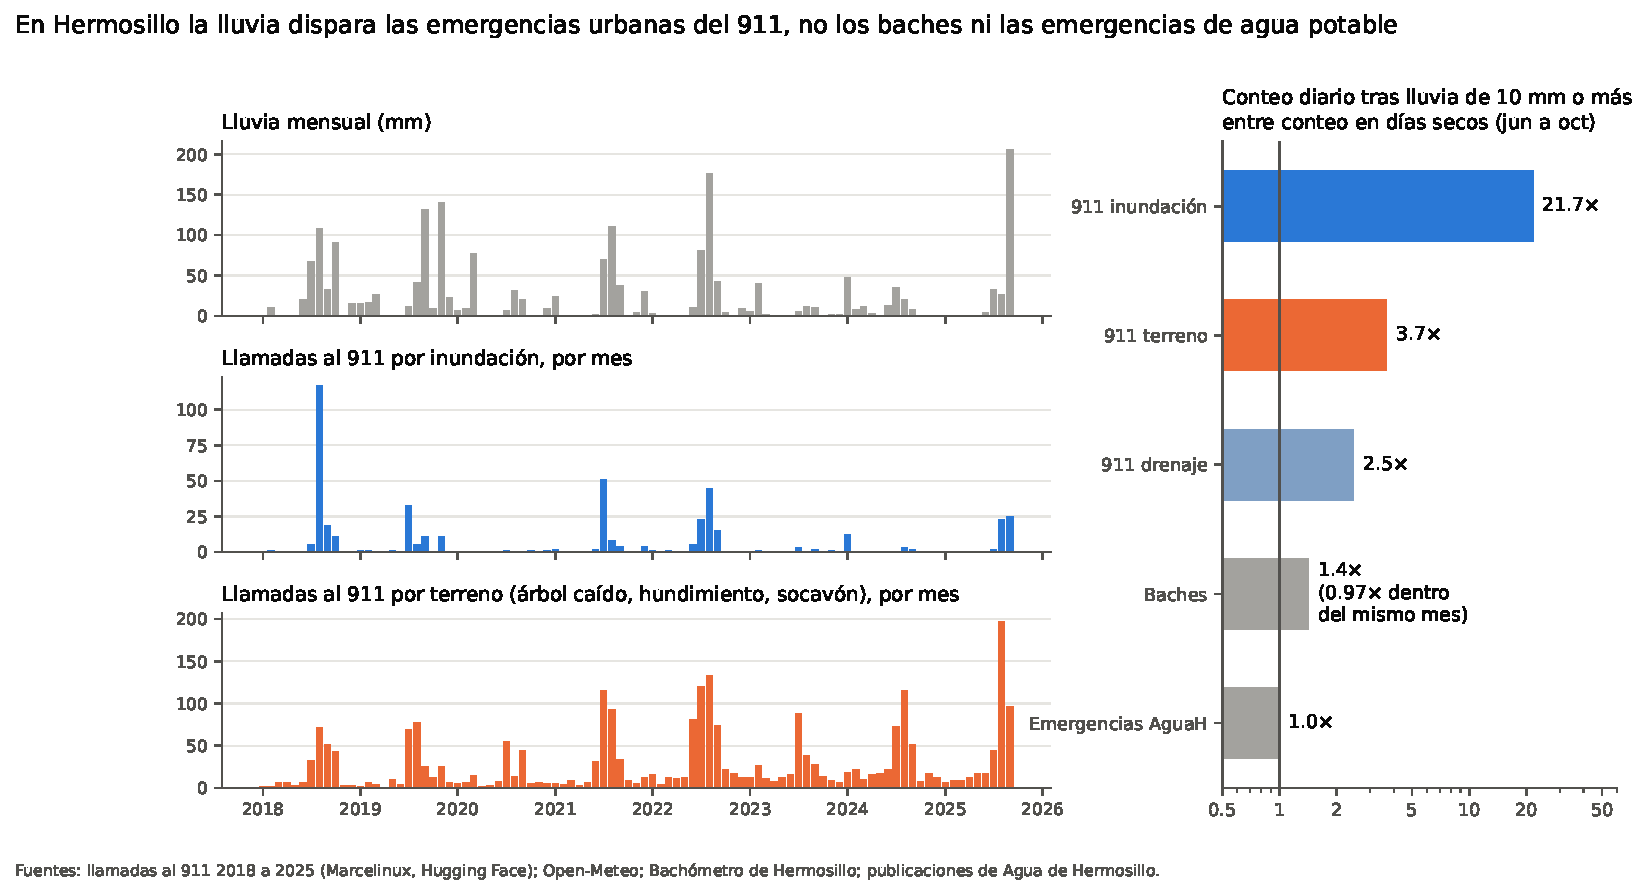
\includegraphics[width=\textwidth]{../img/hallazgo_principal.pdf}
  \caption{Lluvia mensual y llamadas al 911 por inundación y terreno, 2018 a 2025 (izquierda), y razón $Q^{(s)}$ por serie (derecha), de \cod{scripts/figura_hallazgo.py} con las mismas funciones de \cod{water_events.py}.}
  \label{fig:hallazgo}
\end{figure}

Lectura. La correlación es máxima el mismo día y decae en una semana. La razón de temporada separa al 911 (21.70, 3.66 y 2.47) de las fuentes de contraste. El control dentro del mismo mes sostiene la respuesta del 911 (inundación más alta en 14 de 26 meses y más baja en 2; terreno y drenaje en 17 de 26) y borra la de baches: la razón de 1.42 baja a 0.97, con más baches en días húmedos solo en 5 de 12 meses. La razón global de baches reflejaba la tendencia de largo plazo (más reportes cada año) combinada con años recientes más lluviosos. Terreno y drenaje coinciden en la tabla~\ref{tab:e2-mes} en meses y en $Q_{\text{mes}}$ a dos decimales; una verificación de solo lectura con la misma función da 1.522 y 1.524, así que no es un error de copia. A escala anual, los tres años más secos (2020, 2023 y 2024) tienen las cifras más bajas de inundación.

\FloatBarrier
\subsection{E3. Temporada seca}

\begin{table}[!htbp]
  \centering
  \small
  \caption{Emergencias de Agua de Hermosillo por año, porcentaje en abril a junio y publicaciones de pipas (salida \cod{dry_season}).}
  \label{tab:e3}
  \begin{tabular}{lrrr}
    \toprule
    Año & Emergencias & \% en abril a junio & Pipas \\
    \midrule
    2021 & 88 & 29.5 & 2 \\
    2022 & 82 & 22.0 & 0 \\
    2023 & 167 & 48.5 & 0 \\
    2024 & 194 & 17.0 & 29 \\
    2025 & 215 & 22.3 & 6 \\
    \bottomrule
  \end{tabular}
\end{table}

Solo 2023 concentra emergencias en abril a junio; el criterio de 3 de 5 años no se cumple. De las 41 publicaciones de pipas, 28 caen en julio (9) y agosto (19) de 2024 (salida \cod{pipas_months}), después de los dos años más secos de la serie. La escasez aparece como episodio de varios años de sequía, no como temporada anual, y Agua de Hermosillo queda como contexto.

\FloatBarrier
\subsection{E4. Colonias y cauces}

\begin{table}[!htbp]
  \centering
  \small
  \caption{Llamadas ubicadas por grupo y mediana de la distancia $d_c$ al cauce (salida \cod{distance_by_group}).}
  \label{tab:e4-grupo}
  \begin{tabular}{lrr}
    \toprule
    Grupo & Llamadas ubicadas & Mediana al cauce (m) \\
    \midrule
    Ahogamiento & 8 & 1,238 \\
    Drenaje & 730 & 452 \\
    Fenómeno hidrometeorológico & 13 & 178 \\
    Inundación & 293 & 357 \\
    Terreno & 1,752 & 519 \\
    \bottomrule
  \end{tabular}
\end{table}

\begin{table}[!htbp]
  \centering
  \small
  \caption{Cuartiles de distancia al cauce sobre las 314 colonias con llamadas (salida \cod{distance_quartiles}). Spearman por colonia entre el porcentaje de inundación y $d_c$: 0.029.}
  \label{tab:e4-cuartil}
  \begin{tabular}{lrrrr}
    \toprule
    Cuartil de $d_c$ (m) & Colonias & Llamadas & Inundación & \% inundación \\
    \midrule
    1.1 a 114.9 & 79 & 367 & 43 & 11.7 \\
    114.9 a 265.5 & 78 & 485 & 82 & 16.9 \\
    265.5 a 619.7 & 78 & 819 & 80 & 9.8 \\
    619.7 a 2,188.4 & 79 & 1,125 & 88 & 7.8 \\
    \bottomrule
  \end{tabular}
\end{table}

\begin{table}[!htbp]
  \centering
  \small
  \caption{Persistencia entre años: Spearman de las llamadas por colonia (salida \cod{persistence}).}
  \label{tab:e4-persistencia}
  \begin{tabular}{lrr}
    \toprule
    Par de años & Tras lluvia ($M_t\ge\tau$) & Todas las llamadas \\
    \midrule
    2018-2019 & 0.01 & 0.36 \\
    2019-2021 & 0.15 & 0.45 \\
    2021-2022 & 0.16 & 0.51 \\
    2022-2025 & 0.23 & 0.39 \\
    \bottomrule
  \end{tabular}
\end{table}

Lectura. En conjunto, la llamada por inundación viene de una colonia más cercana al cauce que la de terreno (357~m contra 519~m), como en \cod{notebooks/AAMM/07}. Colonia por colonia la relación casi desaparece ($r_s=0.029$) y solo el cuartil más lejano queda claramente abajo. Las llamadas tras lluvia no persisten entre años (0.01 a 0.23), mientras que el total sí persiste (0.36 a 0.51) porque sigue al tamaño de la colonia. El criterio de persistencia no se cumple: la parte espacial queda como descripción.

\FloatBarrier
\subsection{E5. Días anómalos}

Serie: $Y_t$, total diario de inundación, terreno y drenaje del 2018-01-01 al 2025-09-30. Residuo contra la mediana móvil centrada de 29 días,
\[ e_t=Y_t-\operatorname{mediana}(Y_{t-14},\dots,Y_{t+14}), \]
que quita la estacionalidad. Detectores, ninguno con la lluvia como entrada para que el cotejo con la lluvia sea independiente:

\begin{itemize}
  \item Tukey sobre $e_t$, solo del lado alto: anómalo si $e_t>Q_3+k\,(Q_3-Q_1)$ con $k=3$, donde $Q_1$ y $Q_3$ son los cuartiles de $e_t$ (\cod{iqr_outliers}).
  \item IForest \cite{liu2008}, ECOD \cite{li2022} y LOF \cite{breunig2000} de PyOD \cite{zhao2019} (\cod{pyod_outliers}) sobre cuatro variables sin estandarizar: $Y_t$, $e_t$, $\sin(2\pi d/365.25)$ y $\cos(2\pi d/365.25)$, con $d$ el día del año. Parámetros: \cod{contamination=0.01} en los tres; IForest con \cod{random_state=42}; LOF con \cod{n_neighbors=20}; ECOD sin parámetros adicionales.
  \item Votos: número de detectores que marcan el día, de 0 a 4; se revisan los días con 2 votos o más. La coincidencia entre detectores se mide con el índice de Jaccard $J(A,B)=|A\cap B|/|A\cup B|$, con $A$ y $B$ los conjuntos de días marcados.
\end{itemize}

\begin{table}[!htbp]
  \centering
  \small
  \caption{Jaccard entre los conjuntos de días marcados (salida de \cod{agreement_table}).}
  \label{tab:e5-jaccard}
  \begin{tabular}{lrrrr}
    \toprule
     & IForest & ECOD & LOF & Tukey \\
    \midrule
    IForest & 1.00 & 0.61 & 0.04 & 0.33 \\
    ECOD & 0.61 & 1.00 & 0.04 & 0.33 \\
    LOF & 0.04 & 0.04 & 1.00 & 0.02 \\
    Tukey & 0.33 & 0.33 & 0.02 & 1.00 \\
    \bottomrule
  \end{tabular}
\end{table}

\begin{table}[!htbp]
  \centering
  \small
  \caption{Cotejo de los días con 2 votos o más con la lluvia (salida \cod{anomaly_check}).}
  \label{tab:e5-cotejo}
  \begin{tabular}{lr}
    \toprule
    Medida & Valor \\
    \midrule
    Días con 2 votos o más & 36 \\
    \% en julio a septiembre & 83.3 \\
    \% con lluvia de 1~mm o más en los 8 días previos ($M_t\ge\delta$) & 91.7 \\
    \% con lluvia de 10~mm o más en los 8 días previos ($M_t\ge\tau$) & 36.1 \\
    \% de todos los días con $M_t\ge\tau$ & 9.5 \\
    \bottomrule
  \end{tabular}
\end{table}

\begin{table}[!htbp]
  \centering
  \small
  \caption{Los 12 días anómalos con más llamadas (salida \cod{top_days}).}
  \label{tab:e5-top}
  \begin{tabular}{lrrrr}
    \toprule
    Fecha & Llamadas & $R_t$ (mm) & $M_t$ (mm) & Votos \\
    \midrule
    2018-08-12 & 66 & 27.2 & 27.2 & 4 \\
    2022-07-16 & 61 & 12.5 & 12.5 & 4 \\
    2019-07-23 & 47 & 0.1 & 0.8 & 3 \\
    2022-06-29 & 47 & 2.4 & 5.7 & 3 \\
    2021-07-03 & 46 & 4.0 & 4.0 & 3 \\
    2018-10-12 & 46 & 52.4 & 52.4 & 3 \\
    2018-08-18 & 43 & 0.0 & 27.2 & 3 \\
    2023-07-29 & 42 & 1.1 & 1.1 & 3 \\
    2025-09-03 & 40 & 20.3 & 20.3 & 3 \\
    2022-08-18 & 39 & 51.6 & 51.6 & 3 \\
    2025-08-14 & 36 & 4.7 & 4.7 & 3 \\
    2021-07-07 & 35 & 3.2 & 16.1 & 3 \\
    \bottomrule
  \end{tabular}
\end{table}

Lectura. IForest, ECOD y Tukey coinciden entre sí (Jaccard 0.33 a 0.61); LOF marca otros días (0.02 a 0.04) porque busca baja densidad local y no valores extremos. La proporción de días anómalos con $M_t\ge\tau$ (36.1\%) es 3.8 veces la base (9.5\%), pero 63.9\% de los días anómalos no tiene 10~mm en su ventana. Varios días extremos casi no tienen lluvia en la malla (2019-07-23 con 0.1~mm y 2023-07-29 con 1.1~mm), lo esperable si tormentas convectivas locales del monzón \cite{adams1997} no quedan en una malla. E5 valida la relación con la lluvia y a la vez mide el límite principal de la fuente de lluvia.

\FloatBarrier
\subsection{E6. Perfiles de colonia}

Cada colonia con 5 o más llamadas ubicadas (138 colonias) se describe por la participación de cada mes en sus llamadas: una matriz $P\in\mathbb{R}^{138\times 12}$ cuyas filas suman 1. Se ajustó PCA con 4 componentes (\cod{random_state=42}) y se proyectó a 2D con PCA, t-SNE \cite{vandermaaten2008} (perplejidad 20, inicialización PCA, \cod{random_state=42}) y UMAP \cite{mcinnes2018} (\cod{n_neighbors=15}, \cod{min_dist=0.1}, \cod{random_state=42}), con \cod{embed_2d}. La calidad de cada proyección se mide con la confiabilidad (trustworthiness) con $K=10$ vecinos:
\[ T(K)=1-\frac{2}{nK(2n-3K-1)}\sum_{i=1}^{n}\sum_{j\in U_K(i)}\bigl(r(i,j)-K\bigr), \]
donde $n$ es el número de colonias, $U_K(i)$ son los puntos que están entre los $K$ vecinos de $i$ en 2D pero no en el espacio original, y $r(i,j)$ es el rango de $j$ entre los vecinos de $i$ en el espacio original. $T=1$ significa que la proyección no inventa vecinos.

\begin{table}[!htbp]
  \centering
  \small
  \caption{Varianza explicada, cargas principales y confiabilidad de las proyecciones (salidas \cod{pca_variance}, \cod{pca_loadings}, \cod{profile_summary} y \cod{embedding_quality}).}
  \label{tab:e6}
  \begin{tabular}{lr}
    \toprule
    Medida & Valor \\
    \midrule
    Varianza explicada PC1, PC2, PC3, PC4 & 0.331, 0.195, 0.123, 0.072 \\
    Cargas de PC1: julio, agosto, septiembre & $-0.48$, 0.85, $-0.20$ \\
    Cargas de PC2: julio, agosto, septiembre & 0.74, 0.27, $-0.59$ \\
    Spearman de PC1 con la participación de julio a septiembre & 0.15 \\
    Spearman de PC1 con la distancia al cauce & $-0.17$ \\
    Trustworthiness PCA, t-SNE, UMAP & 0.826, 0.878, 0.857 \\
    \bottomrule
  \end{tabular}
\end{table}

Lectura. PC1 no separa colonias lluviosas de colonias planas: contrasta julio con agosto, y PC2 julio con septiembre. Las proyecciones forman una nube continua sin grupos y PC1 apenas se relaciona con la distancia al cauce. Confirma E4: la temporada pega en toda la ciudad y la colonia que llama depende de dónde cayó cada tormenta.

\FloatBarrier
\subsection{E7. Texto}

Se busca la siguiente expresión regular en las descripciones de baches y en el texto más el OCR de Agua de Hermosillo, en minúsculas:
\begin{verbatim}
\bllov|\blluvi|\btormenta|\bchubasc|\baguacer|\bencharc|\binund
\end{verbatim}

\begin{table}[!htbp]
  \centering
  \small
  \caption{Porcentaje de textos de cada mes que mencionan la lluvia (salida \cod{text_by_month}).}
  \label{tab:e7}
  \begin{tabular}{lrrrrrrrrrrrr}
    \toprule
    Mes & 1 & 2 & 3 & 4 & 5 & 6 & 7 & 8 & 9 & 10 & 11 & 12 \\
    \midrule
    Baches & 0.6 & 0.7 & 1.1 & 0.7 & 0.5 & 0.7 & 0.7 & 1.5 & 1.2 & 1.1 & 1.5 & 1.0 \\
    AguaH & 1.6 & 0.2 & 0.0 & 0.8 & 0.0 & 1.0 & 7.0 & 7.5 & 1.9 & 0.7 & 0.6 & 0.0 \\
    \bottomrule
  \end{tabular}
\end{table}

En baches la mención queda entre 0.5\% y 1.5\% sin pico en temporada. En Agua de Hermosillo sube a 7.0\% y 7.5\% en julio y agosto; leídas a mano en el notebook 08, esas publicaciones atribuyen a las tormentas apagones que detienen el bombeo, salidas de operación en El Novillo y pipas de apoyo. La lectura manual no tiene salida tabulada.

\FloatBarrier
\subsection{Resultados operativos del notebook 09}

El notebook 09 traduce E2 a lo que el 911 puede esperar un día de lluvia, con las 4,092 llamadas sin ahogamientos y en la ventana del 911. Las cifras son las salidas guardadas de \cod{notebooks/09-historia-lluvia-911.ipynb}.

\begin{table}[!htbp]
  \centering
  \small
  \caption{Días con 10~mm o más y lluvia anual en la ventana del 911 (salida \cod{rain_days}); 2025 llega a septiembre.}
  \label{tab:n9-dias}
  \begin{tabular}{lrrrrrrrr}
    \toprule
    Año & 2018 & 2019 & 2020 & 2021 & 2022 & 2023 & 2024 & 2025 \\
    \midrule
    Días con $R_t\ge 10$~mm & 10 & 10 & 4 & 9 & 8 & 1 & 2 & 7 \\
    Lluvia (mm) & 348 & 417 & 162 & 279 & 327 & 78 & 148 & 273 \\
    \bottomrule
  \end{tabular}
\end{table}

Salida \cod{summer_share}: 65.3\% de la lluvia y 62.1\% de las llamadas de enero de 2018 a septiembre de 2025 caen en julio a septiembre; el promedio de días con 10~mm o más de 2018 a 2024 es 6.3 por año.

\begin{table}[!htbp]
  \centering
  \small
  \caption{Llamadas del mismo día según la lluvia de ese día, junio a octubre de 2018 a 2025 (salida \cod{intensity}). Día malo: $P_{90}$.}
  \label{tab:n9-intensidad}
  \begin{tabular}{lrrrr}
    \toprule
    Categoría de $R_t$ & Días & Promedio & Día malo & Máximo \\
    \midrule
    Seco ($<1$~mm) & 1,001 & 1.7 & 4.0 & 47 \\
    1 a 10~mm & 155 & 5.1 & 11.0 & 47 \\
    10 a 20~mm & 21 & 9.0 & 18.0 & 61 \\
    20 a 40~mm & 10 & 16.8 & 50.7 & 66 \\
    40~mm o más & 6 & 18.7 & 42.5 & 46 \\
    \bottomrule
  \end{tabular}
\end{table}

\begin{table}[!htbp]
  \centering
  \small
  \caption{Curva de evento $C(k)$ alrededor de los 13 eventos aislados de 20~mm o más (salida \cod{curve}); 6 de los 13 caen en junio a octubre. Día seco de todo el año: 1.04. Con solo los 6 de temporada la curva es demasiado ruidosa para leer una duración.}
  \label{tab:n9-curva}
  \begin{tabular}{lrrrrrrrrrrr}
    \toprule
    $k$ & $-3$ & $-2$ & $-1$ & 0 & 1 & 2 & 3 & 4 & 5 & 6 & 7 \\
    \midrule
    $C(k)$ & 3.69 & 0.69 & 1.77 & 5.77 & 5.77 & 1.92 & 2.69 & 1.31 & 1.08 & 1.38 & 1.54 \\
    \bottomrule
  \end{tabular}
\end{table}

\begin{table}[!htbp]
  \centering
  \small
  \caption{Llamadas por día de cada tipo tras lluvia ($H$) y en días secos ($S$) de junio a octubre, con los nombres cortos de la gráfica; los tipos ya vienen unificados por ortografía (salida de la celda de \cod{type_chart} y de \cod{by_type}).}
  \label{tab:n9-tipos}
  \begin{tabular}{lrrr}
    \toprule
    Tipo & Tras lluvia & Días secos & Extra $x_j$ \\
    \midrule
    Inundación & 1.30 & 0.06 & 1.24 \\
    Árbol caído & 1.92 & 0.70 & 1.22 \\
    Hundimiento & 0.54 & 0.07 & 0.47 \\
    Alcantarilla sin tapa & 0.60 & 0.29 & 0.31 \\
    Derrumbe & 0.29 & 0.02 & 0.27 \\
    Calle en mal estado & 0.28 & 0.07 & 0.21 \\
    Encharcamiento & 0.10 & 0.00 & 0.10 \\
    Socavón & 0.10 & 0.00 & 0.10 \\
    \bottomrule
  \end{tabular}
\end{table}

Perfil por hora (salida \cod{hours}, \cod{night} y \cod{hour_counts}): 554 llamadas en días con $R_t\ge 10$~mm y 1,496 en días secos. La madrugada (1:00 a 5:59) reúne 11.6\% de las llamadas en días de lluvia y 2.7\% en días secos. La hora con más llamadas es las 21:00 en días de lluvia (9.7\%) y las 18:00 en días secos (7.9\%); la salida guardada trunca las columnas de 10 a 13 horas, y una verificación de solo lectura confirma que ninguna supera esos máximos.

Colonias recurrentes (salida \cod{core_summary}): 203 colonias tienen alguna llamada tras lluvia y 50 la tienen en 3 años calendario o más; esas 50 reúnen 61.8\% de las llamadas ubicadas tras lluvia. Su área mediana es 0.56~km$^2$, contra 0.08~km$^2$ de todas las colonias. Las cinco con más llamadas (salida \cod{core_list}) son San Benito (44 llamadas, 6 años), Balderrama (26, 6), Sahuaro (19, 6), Olivares (19, 4) y Centro (17, 4).

\begin{table}[!htbp]
  \centering
  \small
  \caption{Razón por serie: toda la temporada ($Q^{(s)}$) y dentro del mismo mes ($Q_{\text{mes}}$) (salida \cod{not_rain}). En inundación y Agua de Hermosillo no se calcula $Q_{\text{mes}}$ en este notebook; el de inundación está en la tabla~\ref{tab:e2-mes}.}
  \label{tab:n9-nolluvia}
  \begin{tabular}{lrr}
    \toprule
    Serie & Temporada & Mismo mes \\
    \midrule
    911 inundación & 21.70 & \\
    911 terreno & 3.66 & 1.52 \\
    911 drenaje & 2.47 & 1.52 \\
    Baches & 1.42 & 0.97 \\
    Emergencias AguaH & 0.99 & \\
    \bottomrule
  \end{tabular}
\end{table}

\begin{figure}[!htbp]
  \centering
  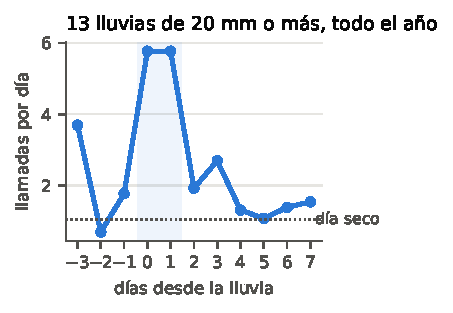
\includegraphics[width=0.36\textwidth]{../img/historia/3_dos_dias.pdf}
  \caption{Curva de evento $C(k)$ de la tabla~\ref{tab:n9-curva}, del notebook 09; punteado: día seco de temporada.}
  \label{fig:curva}
\end{figure}

\section{Decisiones y descartes}
\label{sec:decisiones}

\subsection{Por qué la pregunta se redefinió hacia el 911}

Los EDA por dataset (notebooks 05 a 07 y \cod{notebooks/AAMM/}) cumplieron las secciones del curso pero no compartían una pregunta. La pregunta candidata del notebook 08 preguntaba cuándo y dónde se concentran las afectaciones ligadas al agua y cuánto explican la lluvia y los cauces. Las exploraciones decidieron su forma final:

\begin{itemize}
  \item E1 y E2 se cumplen para el 911: concentración en julio a septiembre todos los años y respuesta a la lluvia que sobrevive al control dentro del mismo mes. El 911 pasa a ser la serie principal y la parte diagnóstica es el estudio de evento.
  \item E1, E2 y E3 no se cumplen para baches ni para Agua de Hermosillo: sin estacionalidad de julio a septiembre, sin respuesta dentro del mismo mes (0.97) o en la temporada (0.99), y sin temporada seca recurrente. Quedan como contraste: muestran que el pronóstico de lluvia no sirve para esos servicios.
  \item E4 y E6 no sostienen un diagnóstico espacial: la parte de ``en qué colonias'' es descriptiva, por temporada, sin atribuirla a la cercanía al cauce.
  \item E5 y E7 aportan validación y evidencia cualitativa, y exponen el límite de la fuente de lluvia.
\end{itemize}

Pregunta redefinida: ¿cuánto aumentan las emergencias urbanas reportadas al 911 en Hermosillo cuando llueve, qué tipos de incidente responden y en qué colonias se concentran en cada temporada de lluvias?

\FloatBarrier
\subsection{Qué se consolidó y qué se desechó de los EDA previos}

\begin{table}[!htbp]
  \centering
  \footnotesize
  \caption{Elementos de los EDA previos y su destino (\cod{docs/redefinicion.md}).}
  \label{tab:descartes}
  \begin{tabularx}{\textwidth}{L{4.6cm} L{3.6cm} Y}
    \toprule
    Elemento & Origen & Decisión y motivo \\
    \midrule
    Estacionalidad del 911 por grupo & \cod{notebooks/AAMM/07} & Se consolida; el notebook dice agosto a octubre y el código usa julio a septiembre \\
    Distancia al cauce por grupo de incidente & \cod{notebooks/AAMM/07} & Se consolida; reproducida en E4 (357~m contra 519~m) \\
    Cruce espacial de baches a colonia & \cod{add_colonia_bache_with_gpkg.py} & Se conserva para el tablero; los baches salen de la pregunta \\
    Salto de julio a agosto en baches & \cod{docs/cinco_v_datos.md} & Se desecha como señal de lluvia: julio es el mes más bajo \\
    Hipótesis de lluvia para emergencias de Agua de Hermosillo & \cod{notebooks/AAMM/06} & Se desecha: razón 0.99 \\
    Episodios de interacción en Agua de Hermosillo & \cod{notebooks/05}, celda 27 & Contexto para etiquetar eventos en el tablero \\
    Sectores Norte, Centro y Sur & \cod{notebooks/AAMM/05} & Solo agrupador; la etiqueta de latitud (27.3 N) es errónea \\
    Correlaciones por construcción (\cod{likes_count} con \cod{reactions_total}, \cod{n_posts} con \cod{n_mentions}, \cod{ORDER_1} con \cod{ARBSUM_1}) & notebooks 05 a 07, AAMM 06 y 09 & Se desechan: miden la misma cantidad \\
    t-SNE y UMAP de interacción y de huella & notebooks 05 y 07 & Se desechan: los grupos los define la codificación de entrada \\
    Tasa por clase de cercanía & \cod{notebooks/AAMM/08}, celda 25 & Se desecha: divide entre el área de todo el sector \\
    K-Means sobre distancias & \cod{notebooks/AAMM/08} y 09 & Se desecha: distancias colineales; el grupo repite el sector \\
    Kruskal-Wallis sobre llamadas & \cod{notebooks/AAMM/07} & Se desecha: filas no independientes \\
    Cruce de baches por nombre de colonia & \cod{add_colonia_name_to_bache_job.py} & Se desecha: salida nula en todas las filas \\
    Tukey sobre \cod{top_comment_likes} & \cod{notebooks/05} & Se desecha: dos de cada tres valores son cero \\
    \bottomrule
  \end{tabularx}
\end{table}

\section{Trazabilidad de las cifras del reporte ejecutivo}
\label{sec:traza}

Cada fila es una cifra o afirmación cuantitativa de \cod{docs/reporte/reporte.tex}, con el notebook (08 o 09), la variable que guarda la salida y la función de \cod{water_events.py} que la calcula. Estado: ``rastreada'' si la cifra está en una salida guardada; ``derivada'' si es una operación simple sobre salidas guardadas; las demás filas explican qué falta. La segunda columna cita el ejecutivo con su propio redondeo.

\footnotesize
\begin{longtable}{L{0.4cm} L{4.2cm} L{4.0cm} L{2.4cm} L{4.0cm}}
  \caption{Trazabilidad de las cifras del reporte ejecutivo.}\label{tab:traza}\\
  \toprule
  \# & Cifra en el ejecutivo & Origen & Valor en la salida & Estado \\
  \midrule
  \endfirsthead
  \toprule
  \# & Cifra en el ejecutivo & Origen & Valor en la salida & Estado \\
  \midrule
  \endhead
  \bottomrule
  \endfoot
  1 & Lluvia de 10~mm o más unas seis veces al año & nb09, \cod{summer_share}; \cod{rain_days} & 6.3 (promedio 2018 a 2024) & Rastreada \\
  2 & Dos de cada tres veces de julio a septiembre (días de 10~mm o más) & nb09, \cod{summer_share} & 34 de 51 días (2018-01 a 2025-09) & Rastreada \\
  3 & Día seco de temporada: 1.7 llamadas de los tipos ligados al agua y al terreno & nb09, \cod{intensity} (\cod{calls_by_intensity}) & 1.7 (1,001 días) & Rastreada; todos los tipos del filtro salvo ahogamientos \\
  4 & Con 10 a 20~mm llegan 9 & nb09, \cod{intensity} & 9.0 (21 días) & Rastreada \\
  5 & Con más de 20~mm entre 17 y 19 & nb09, \cod{intensity} & 16.8 (10 días) y 18.7 (6 días) & Rastreada \\
  6 & Días malos de más de 40 & nb09, \cod{intensity}, columna \cod{dia_malo} & 50.7 y 42.5 & Rastreada; vale para más de 20~mm \\
  7 & Tras una tormenta fuerte, el día siguiente recibe tantas llamadas como el de la lluvia, unas cinco veces un día seco & nb09, \cod{curve} (\cod{event_curve}) & $C(0)=C(1)=5.77$, $C(2)=1.92$; día seco del año 1.04 & Rastreada; 5.77/1.04 = 5.5 \\
  8 & Sobre todo árboles e inundaciones & nb09, celda de \cod{type_chart}; \cod{by_type} & extra 1.22 y 1.24 & Rastreada \\
  9 & Crece de madrugada & nb09, \cod{night} (\cod{hour_profile}) & 11.6\% contra 2.7\% & Rastreada \\
  10 & Ante 20~mm o más, unas diez veces un día seco, y alta también al día siguiente & nb09, \cod{intensity} y \cod{curve} & 16.8/1.7 y 18.7/1.7; $C(1)=5.77$ & Derivada \\
  11 & 50 colonias en tres años o más, 62\% de las llamadas ubicadas & nb09, \cod{core_summary} (\cod{seasons_with_calls}) & 50; 61.8\% & Rastreada; proporción de las llamadas ubicadas tras lluvia \\
  12 & San Benito, Balderrama, Sahuaro, Olivares y Centro & nb09, \cod{core_list} & 44, 26, 19, 19 y 17 llamadas & Rastreada \\
  13 & Baches y agua potable no aumentan con la lluvia & nb08, \cod{within_month} y \cod{event_table}; nb09, \cod{not_rain} & 0.97 (mismo mes); 0.99 & Rastreada \\
  14 & Figura 1: un día malo, 1 de cada 10 días lo supera & nb09, \cod{calls_by_intensity} & $P_{90}$ & Rastreada (definición) \\
  15 & Tabla 1: llamadas al 911, 2018 a 2025 & nb08, \cod{coverage_table} & 2018-01-05 a 2025-09-30 & Rastreada \\
  16 & Dos tercios de la lluvia del año de julio a septiembre & nb09, \cod{summer_share} & 65.3\% & Rastreada \\
  17 & En esos meses entra la mayor parte de las llamadas & nb09, \cod{summer_share} & 62.1\% & Rastreada \\
  18 & En 2023 y 2024 las llamadas por inundación casi desaparecen & nb08, \cod{calls_by_year}; \cod{annual} & 7 y 17 & Rastreada \\
  19 & Cada escalón de lluvia sube el promedio & nb09, \cod{intensity} & 1.7, 5.1, 9.0, 16.8, 18.7 & Rastreada \\
  20 & Hasta unas diez veces un día seco con más de 20~mm & nb09, \cod{intensity} & 16.8/1.7 = 9.9; 18.7/1.7 = 11.0 & Derivada \\
  21 & Figura del calendario: enero de 2018 a septiembre de 2025 & nb09, \cod{monthly} & ventana del 911 & Rastreada \\
  22 & Siguen hundimientos, alcantarillas sin tapa y derrumbes & nb09, celda de \cod{type_chart} & extra: 0.47, 0.31 y 0.27 & Rastreada \\
  23 & El pico pasa de las 18:00 a las 21:00 & nb09, \cod{hours} & 7.9\% a las 18:00 seco; 9.7\% a las 21:00 lluvia & Rastreada \\
  24 & La madrugada recibe 12\%, cuatro veces lo de un día seco & nb09, \cod{night} & 11.6\% contra 2.7\%; 11.6/2.7 = 4.3 & Rastreada y derivada \\
  25 & Se ubicaron dos de cada tres llamadas & nb08, \cod{quality_table} & 67.0\% & Rastreada \\
  26 & Las colonias afectadas cambian de un año a otro & nb08, \cod{persistence} & 0.01 a 0.23 & Rastreada \\
  27 & Colonias grandes, área mediana siete veces la del conjunto & nb09, \cod{core_summary} & 0.56 contra 0.08~km$^2$ & Derivada; 0.56/0.08 = 7 \\
  28 & Inundación sube 21.7 veces & nb08, \cod{event_table}; nb09, \cod{not_rain} & 21.70 & Rastreada \\
  29 & La lluvia aparece en el texto de Agua de Hermosillo como causa de apagones & nb08, \cod{text_by_month} y lectura manual & 7.0\% y 7.5\% en julio y agosto & Porcentajes rastreados; la atribución a apagones es lectura manual sin salida tabulada \\
  30 & Una de cada tres llamadas no se ubicó & nb08, \cod{quality_table} & 100 $-$ 67.0 = 33.0\% & Derivada \\
  31 & Agua de Hermosillo de diciembre de 2020 a septiembre de 2026 & nb08, \cod{coverage_table} & 2020-12-07 a 2026-09-14 & Rastreada \\
\end{longtable}
\normalsize

\section{Limitaciones y amenazas a la validez}
\label{sec:limites}

\begin{itemize}
  \item Resolución de la lluvia. Es un punto de una malla de reanálisis, no una estación, y no se confirmó el modelo. 63.9\% de los días anómalos de E5 no tiene 10~mm en su ventana, y hay días con más de 40 llamadas y casi 0~mm. Las razones y promedios por categoría tienden a quedarse cortos: días con tormenta local quedan clasificados como secos o de lluvia ligera.
  \item Emparejamiento por nombre. 33.0\% de las llamadas no se ubica; los 18 nombres repetidos en la ciudad se excluyen aunque la llamada sea de una de esas colonias; un error de captura no se corrige. Si las colonias que no se ubican difieren de las que sí, el mapa y la lista de colonias recurrentes tienen sesgo.
  \item Sin población por colonia. Los conteos por colonia no son tasas: las colonias recurrentes tienen área mediana 0.56~km$^2$ contra 0.08~km$^2$, y el total por colonia persiste entre años porque sigue al tamaño.
  \item Pocos días de lluvia fuerte. En junio a octubre de 2018 a 2025 hay 21 días de 10 a 20~mm, 10 de 20 a 40~mm y 6 de 40~mm o más; la curva de evento usa 13 eventos. El percentil 90 sobre 6 o 10 días es inestable (en la tabla~\ref{tab:n9-intensidad} el día malo de 20 a 40~mm supera al de 40~mm o más).
  \item Filas no independientes. Los conteos diarios tienen autocorrelación y las ventanas de 8 días se traslapan, así que un mismo día puede contar para varias lluvias. No se reportan intervalos ni pruebas de hipótesis; por la misma razón se desechó el Kruskal-Wallis de los EDA previos. Las razones son descriptivas.
  \item Definiciones que no se limitan a la temporada. La curva de evento usa eventos de todo el año (7 de 13 fuera de junio a octubre) y por eso se compara con el día seco de todo el año; \cod{seasons_with_calls} y \cod{hour_profile} usan todos los meses; el control dentro del mismo mes compara todos los meses del año. Las cifras de la historia mezclan, por tanto, lluvias de verano con lluvias invernales.
  \item Dos definiciones de día seco: $R_t<\delta$ el mismo día (tabla~\ref{tab:n9-intensidad}, 1,001 días) y $M_t<\delta$ en la ventana de 8 días (tabla~\ref{tab:e2-evento}, 586 días). El 1.7 del ejecutivo usa la primera.
  \item Catálogo del 911. Selección manual de 34 cadenas de 475, unificadas en 28 tipos; la selección es un juicio del equipo; \cod{fenomeno_hidrometeorologico} solo existe en 2025.
  \item Red hidrográfica 1:50\,000 con segmentos de 1998 a 2010 y sin drenaje pluvial urbano; la distancia es del centroide de la colonia, no del lugar de la llamada.
  \item Baches: los conteos incluyen 511 puntos fuera del recuadro de la ciudad y 152 repetidos.
\end{itemize}

\section{Reproducibilidad}
\label{sec:repro}

Comandos, desde la raíz del repositorio:

\begin{enumerate}
  \item \texttt{uv sync} instala el entorno de \cod{pyproject.toml} y \cod{uv.lock}.
  \item Descargar el snapshot de \cod{data/external} (\cod{data/SNAPSHOT.md}), descomprimirlo en \cod{data/} y correr \texttt{make verify-data}.
  \item \texttt{make data}: corre \texttt{make download} (los seis jobs de ingesta en paralelo, cada uno con su \cod{FUENTE.txt} y sha256), los jobs de procesamiento y \cod{validate_data_job}.
  \item \texttt{make nb NOTEBOOK=08-exploracion-redefinicion} y \texttt{make nb NOTEBOOK=09-historia-lluvia-911}: exportan los notebooks marimo a \cod{.ipynb} con salidas; el 09 escribe las figuras de \cod{docs/img/historia/}.
  \item \texttt{uv run python scripts/figura\_hallazgo.py}: figura~\ref{fig:hallazgo}.
  \item \texttt{make test}: pruebas, incluidas las de los jobs de precipitación y la unificación de tipos del 911.
\end{enumerate}

Parámetros. En \cod{params.yml}: URL, punto, periodo, variables y zona horaria de Open-Meteo (\cod{sources.open_meteo.datasets.precipitacion_hermosillo.query}); URL y rutas del 911 (\cod{sources.llamadas911}); años del Bachómetro; rutas de cada dataset. En \cod{project_name/water_events.py}: \cod{COVERAGE}, \cod{RAIN_EVENT_MM} = 10, \cod{RESPONSE_DAYS} = 8, \cod{DRY_MM} = 1, \cod{RAINY_MONTHS} = 6 a 10, \cod{EVENT_MM} = 20, \cod{INTENSITY_BINS}, \cod{METRIC_CRS} = EPSG:6372, \cod{CITY_LOCALITY} = 0001 y el buffer de 5~km. En \cod{project_name/features.py}: \cod{GRUPOS_INCIDENTE_911}.

Semillas. \cod{RANDOM_STATE} = 42 en \cod{project_name/eda.py} para IForest, PCA, t-SNE y UMAP; el PCA de E6 usa \cod{random_state=42}. ECOD, LOF y Tukey son deterministas.

\begin{table}[!htbp]
  \centering
  \small
  \caption{Versiones de software (\cod{uv.lock} y \cod{.venv}).}
  \label{tab:versiones}
  \begin{tabular}{llll}
    \toprule
    Paquete & Versión & Paquete & Versión \\
    \midrule
    Python & 3.13.12 & scipy & 1.18.1 \\
    pandas & 3.0.5 & geopandas & 1.1.4 \\
    numpy & 2.3.5 & shapely & 2.1.2 \\
    scikit-learn & 1.9.1 & pyproj & 3.8.0 \\
    pyod & 3.6.7 & pyogrio & 0.13.0 \\
    umap-learn & 0.5.12 & python-calamine & 0.9.0 \\
    marimo & 0.24.0 & pandera & 0.33.1 \\
    matplotlib & 3.11.1 & ydata-profiling (entorno aislado) & 4.18.4 \\
    \bottomrule
  \end{tabular}
\end{table}

Advertencias de reproducción:

\begin{itemize}
  \item \cod{schemas.py} no tiene reglas para el 911, la precipitación ni los baches; \texttt{make validate} no los revisa.
  \item La política de descarga es \cod{skip}: si el archivo crudo existe no se vuelve a bajar. El Bachómetro vuelve a bajar el año en curso: el crudo actual (descarga del 3 de octubre de 2026) tiene 39,106 reportes y el \cod{baches_hermosillo.csv} procesado (28 de septiembre de 2026), con el que se calcularon las salidas, tiene 39,018; correr \texttt{make data} hoy cambia las cifras de baches.
  \item El snapshot de Facebook no se puede regenerar (scraper de paga, URLs que expiran, OCR dependiente de hardware); solo se verifica con sus checksums.
\end{itemize}

\begin{thebibliography}{99}
\raggedright

\bibitem{adams1997}
Adams, D. K. y Comrie, A. C. (1997). The North American Monsoon. Bulletin of the American Meteorological Society, 78(10), 2197-2213. \url{https://doi.org/10.1175/1520-0477(1997)078<2197:TNAM>2.0.CO;2}

\bibitem{aguah}
Agua de Hermosillo. Publicaciones de la página oficial de Facebook, diciembre de 2020 a septiembre de 2026. Snapshot descrito en \cod{data/SNAPSHOT.md}.

\bibitem{breunig2000}
Breunig, M. M., Kriegel, H.-P., Ng, R. T. y Sander, J. (2000). LOF: Identifying Density-Based Local Outliers. Proceedings of the ACM SIGMOD International Conference on Management of Data, 93-104. \url{https://doi.org/10.1145/342009.335388}

\bibitem{bachometro}
H. Ayuntamiento de Hermosillo. Bachómetro. \url{https://bachometro.hermosillo.gob.mx}

\bibitem{inegidcah}
INEGI (2025). Delimitación de colonias y otros asentamientos humanos (DCAH). \url{https://www.inegi.org.mx/programas/dcah/}

\bibitem{inegired}
INEGI. Red Hidrográfica escala 1:50 000, edición 2.0. \url{https://www.inegi.org.mx/temas/hidrografia/}

\bibitem{li2022}
Li, Z., Zhao, Y., Hu, X., Botta, N., Ionescu, C. y Chen, G. H. (2022). ECOD: Unsupervised Outlier Detection Using Empirical Cumulative Distribution Functions. IEEE Transactions on Knowledge and Data Engineering. \url{https://doi.org/10.1109/TKDE.2022.3159580}

\bibitem{liu2008}
Liu, F. T., Ting, K. M. y Zhou, Z.-H. (2008). Isolation Forest. IEEE International Conference on Data Mining, 413-422. \url{https://doi.org/10.1109/ICDM.2008.17}

\bibitem{marcelinux2025}
Marcelinux (2025). Llamadas 911 por colonia, Hermosillo 2018-2025. Hugging Face, CC-BY-4.0. \url{https://huggingface.co/datasets/Marcelinux/llamadas911_colonias_hermosillo_2018_2025}

\bibitem{mcinnes2018}
McInnes, L., Healy, J. y Melville, J. (2018). UMAP: Uniform Manifold Approximation and Projection for Dimension Reduction. arXiv:1802.03426.

\bibitem{munozsabater2021}
Muñoz-Sabater, J. et al. (2021). ERA5-Land: a state-of-the-art global reanalysis dataset for land applications. Earth System Science Data, 13, 4349-4383. \url{https://doi.org/10.5194/essd-13-4349-2021}. Es uno de los reanálisis que combina Open-Meteo; no se confirmó que sea el que usa para el punto de Hermosillo.

\bibitem{vandermaaten2008}
van der Maaten, L. y Hinton, G. (2008). Visualizing Data using t-SNE. Journal of Machine Learning Research, 9, 2579-2605.

\bibitem{zhao2019}
Zhao, Y., Nasrullah, Z. y Li, Z. (2019). PyOD: A Python Toolbox for Scalable Outlier Detection. Journal of Machine Learning Research, 20(96), 1-7.

\bibitem{zippenfenig2023}
Zippenfenig, P. (2023). Open-Meteo.com Weather API. Zenodo. \url{https://doi.org/10.5281/zenodo.7970649}

\end{thebibliography}

\end{document}
